\documentclass[xcolor={dvipsnames}]{beamer}

% allowing font sizes at arbitrary sizes
\usepackage{lmodern}

\usetheme{Madrid}
%\usecolortheme{whale}
% define my color
\definecolor{mycolor}{RGB}{2,105,164}
\setbeamercolor{titlelike}{parent=structure, fg=white, bg=mycolor}
\usefonttheme{}

\usepackage{mathtools, amsmath, amssymb, subfigure, multicol, amsthm}
\usepackage{graphicx}
\usepackage{caption}
\usepackage{algorithm2e}
\captionsetup{skip=0.5pt}
%\usepackage{subcaption}
%\usepackage{enumitem}
% set Reference as a section
\usepackage[numberedbib]{apacite}

\usepackage{mathrsfs}
\usepackage{tikz}

\usepackage{soul}

%\usepackage{algcompatible}
%\usepackage[ruled,vlined]{algorithm2e}
%\usepackage{algpseudocode}

\usepackage{chronosys}%创建时间轴

\usepackage{threeparttable}

% \useshortspace
\usepackage{nccmath}

% tables
\usepackage{booktabs}
\usepackage[normalem]{ulem}
\useunder{\uline}{\ul}{}

\usepackage{makecell}

\usepackage{etex}


\hypersetup{
    colorlinks,
    citecolor=mycolor,
    linkcolor=mycolor
}


\bibliographystyle{apacite}


\theoremstyle{plain}
\newtheorem{prop}{Proposition}

%matrix notation
\newcommand{\matr}[1]{\mathbf{#1}} % undergraduate algebra version
%gets rid of top navigation bars
\setbeamertemplate{headline}{}
%gets rid of bottom navigation bars
\setbeamertemplate{footline}[frame number]{}
%gets rid of bottom navigation symbols
\setbeamertemplate{navigation symbols}{}
%no number in frame title
\setbeamertemplate{frametitle continuation}{}

% propositions
\setbeamertemplate{definitions}[ams style]
\setbeamertemplate{theorems}[ams style]

\newcommand{\RomanNumeralCaps}[1]{\MakeUppercase{\romannumeral #1}}

\makeatletter
\renewcommand\eqref[1]{%
  \textup{\usebeamercolor[fg]{structure}\tagform@{\ref{#1}}}%
}

\usepackage{datetime} % month-year format
\newdateformat{monthyeardate}{%
  \monthname[\THEMONTH], \THEYEAR}

% graphs and tables paths
\newcommand{\graphs}{../../Graphs}
\newcommand{\tables}{../../Tables}

% set the color and shape of subitem
%\setbeamertemplate{itemize item}[circle]
\setbeamertemplate{itemize subitem}[triangle]
%\setbeamercolor{itemize subitem}{fg=cyan}
\setbeamertemplate{enumerate items}[default]
\setbeamertemplate{itemize subsubitem}[square]
% set number of table
\setbeamertemplate{caption}[numbered]
%equation 2.1, 2.2......
%\numberwithin{equation}{section}

\def\sym#1{\ifmmode^{#1}\else\(^{#1}\)\fi}

\title{\Large{Land Offers and Fiscal Competition Between City Governments in China}}

% \author{Wending Liu\texorpdfstring{\\}{Lg}Supervisor: Fedor Iskhakov}
\author{Wending Liu}
\institute{ANU Research School of Economics}
\centering
\date{Econometric Society Australasian Meeting\\\monthyeardate\today}

\makeatletter
\let\@@magyar@captionfix\relax
\makeatother

\usepackage{amsmath}
\DeclareMathOperator*{\argmax}{arg\,max}
\DeclareMathOperator*{\argmin}{arg\,min}
\DeclareMathOperator{\Var}{Var}
\DeclareMathOperator{\AVar}{AVar}

\begin{document}
\maketitle


\section{Motivation}
\begin{frame}{Motivation}
    \begin{itemize}
        \item China's governance structure is unusual in combining a high degree of
              political centralization and economic decentralization \\
              (\citeNP{kroeber2020china}; \citeNP{xu2011fundamental}).
        \item One of the most salient characteristics of the system is
              the competition among city governments which use special deals to attract businesses
              \cite{bai2020special}.
        \item A major type of the special deals is
              selling industrial lands at a low price to firms.
              \cite{su2017china}
        \item Why local governments in China compete against each other
              to attract industrial firms so fiercely that they are willing to sacrifice the industrial
              land selling revenue?
        \item What and how much are the benefits city governments
              can get from this kind of fiscal competition?
        \item Can this kind of fiscal competition improve the allocation efficiency or
              does it lead to ``race to bottom''?
        \item Can this kind of fiscal competition continue in the future?
    \end{itemize}
\end{frame}

\begin{frame}{Motivation}
    \begin{figure}[htbp]
        \centering
        \begin{minipage}[t]{0.48\textwidth}
            \centering
            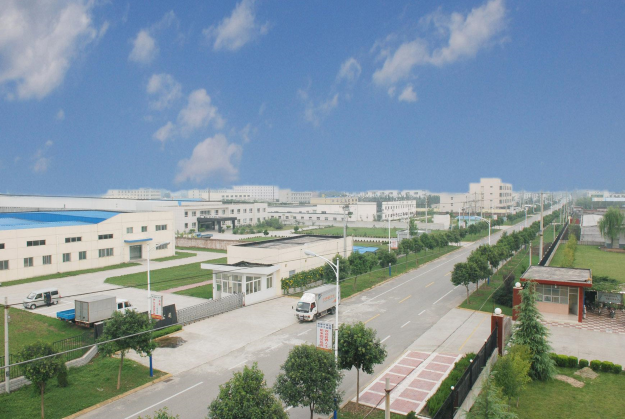
\includegraphics[scale=0.33]{\graphs/industrial park.png}
            \caption*{An industrial park in the author's hometown}
            \label{industrial park}
        \end{minipage}
        \begin{minipage}[t]{0.48\textwidth}
            \centering
            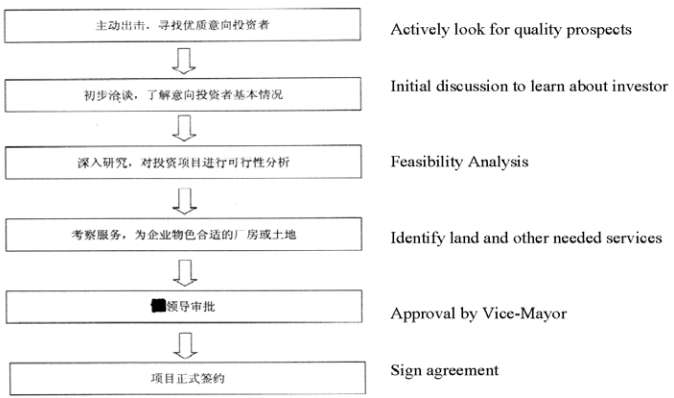
\includegraphics[scale=0.35]{\graphs/workflow.png}
            \caption*{Work program of a vice-mayor (who takes charge of education!) in China \cite{bai2020special}}
            \label{workflow}
        \end{minipage}
    \end{figure}
\end{frame}

\section{Literature Review}
\begin{frame}{Literature Review}
    \begin{itemize}

        \item Fiscal Competition Theory
              \begin{itemize}
                  \item Tiebout Model: competition for mobile capitals creates efficient equilibrium
                        \cite{tiebout1956pure}.
                  \item Tax competition Model: downward pressure on fiscal revenues
                        from the decentralization of fiscal power
                        \cite{keen1997fiscal}.
                  \item The possibilities of a ``race to bottom" in welfare benefits
                        due to ``fiscal externality" \cite{wilson1999theories}.
              \end{itemize}
        \item Fiscal Competition with Chinese characteristics
              \begin{itemize}
                  \item Studies observe that local governments use discounts in
                        land sale as a main tool
                        to attract businesses include \citeA{cheung2014economic},
                        \citeA{su2017china}, \citeA{bai2020special}, etc.
                  \item No formal theoretical model and econometric analysis yet.
              \end{itemize}
        \item Empirical Analysis
              \begin{itemize}
                  \item \citeA{mast2020race} uses structural estimation to
                        analyze the county tax break for small businesses in the U.S.
              \end{itemize}
    \end{itemize}
\end{frame}

% %outline of paper
% \begin{frame}
%     \frametitle{Roadmap}
%     \tableofcontents
% \end{frame}

\section{Fiscal Competition and Land Market in China}
\begin{frame}{Fiscal Competition and Land Market in China}
    \begin{itemize}
        \item City governments (293 prefecture-level cities + 4 municipalities) control the land supply.
        \item Land revenue represented 30\% of the total government revenue and 6\% of total GDP by 2011
              \cite{chen2019busting}.
        \item But interestingly, the price of industrial land is significantly
              lower than the price of residential land.
              \begin{figure}
                  \centering
                  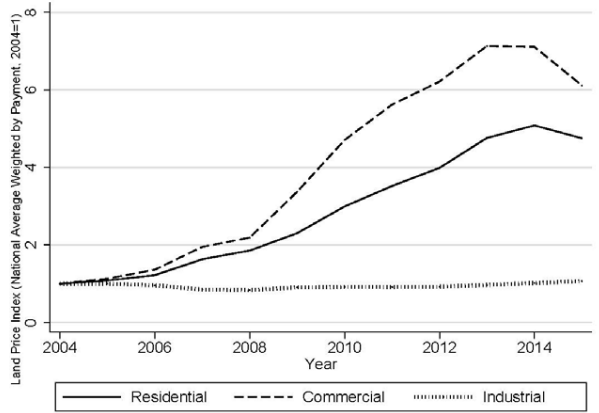
\includegraphics[scale=0.42]{\graphs/land_price_index.png}
                  \caption*{\footnotesize
                      {Land price index in China
                          (Source: \citeA{LiuXiong+2020+183+207})}}
                  \label{land price}
              \end{figure}
    \end{itemize}
\end{frame}


\begin{frame}{Fiscal Competition and Land Market in China}
    \begin{itemize}
        \item The reason behind the seemingly confusing phenomenon is deeply rooted
              in the fiscal structure of Chinese local governments.
        \item After the tax reform in 1993-1994,
              the main source of local government's fiscal revenue comes from
              25\% of value-added tax, business tax,
              and 40\% of income tax plus the land lease fees.
        \item To maximize fiscal revenue, local governments use special deals to
              attract industrial firms.
              And a major type of special deals is to sell industrial lands
              at a very low price to firms.
        \item Why industrial firms are so important for local governments?
              \begin{itemize}
                  \item more (industrial) firms
                        $\rightarrow$ more workers
                        $\rightarrow$ prosperity of the tertiary industry
                        $\rightarrow$ increasing housing demand and tax revenue.
                  \item City governments can maximize their revenues
                        by limiting residential land supply given the increasing housing demand.
              \end{itemize}
        \item This paper focuses on fiscal competition,
              i.e. attracting firms by lowering the land price,
              as well as its impact on fiscal revenue.
    \end{itemize}
\end{frame}


\section{The Model}
\subsection{Main structure of the model}
\begin{frame}{Main structure of the model}
    \begin{figure}
        \centering
        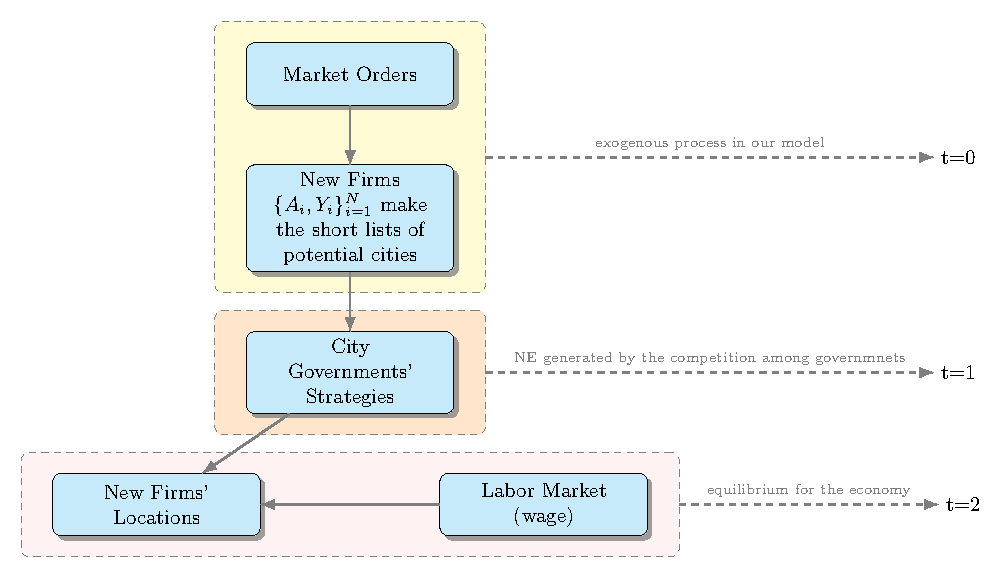
\includegraphics[scale=0.7]{\graphs/timing/timing.pdf}
        %\caption*{Main structure of the model (solid arrows represent causal channels)}
        \label{fig3}
    \end{figure}
\end{frame}


\subsection{Firms}
\begin{frame}{Firms}
    \begin{itemize}
        \item Firm $i$'s (Leontief) production function:
              $$
                  F_{i}(K,L,T) = \min\{A_{i} K^{\alpha}L^{1-\alpha}, g_{i}(T)\}
              $$
              where $T$ is the area of industrial land, which determines the limit of output.
              $g_i(T)$ is increasing in $T$.
        \item New firm $i$ signs a contract to produce $Y_i$ units of product with buyers
              on the global market.
              The price of product is normalized to 1 RMB.
        \item Firm $i$ solves the following cost minimization problem:
              \begin{equation}
                  \begin{aligned}
                       & \min _{k \in \mathbf{C}_{i}, K_{i}, L_{i}, T_{i}}
                      \left\{r K_{i}+w_{k} L_{i}+\frac{p_{i k}}{m} T_{i}-\varepsilon_{i k}\right\}     \\
                       & \text { s.t. } Y_{i}=\min \left\{A_{i} K_{i}^{\alpha} L_{i}^{1-\alpha}, g_{i}
                      \left(T_{i}\right)\right\}
                  \end{aligned}
                  \label{firm_minimization1}
              \end{equation}
              \begin{itemize}
                  \item $p_{ik}$: land price for firm $i$ offered by city $k$.
                  \item $m$: term (years) of land lease.
                  \item $\mathbf{C}_i$: firm $i$'s choice set. $|\mathbf{C}_i|$ is
                        nondecreasing in $Y_i$.
                  \item $\varepsilon_{ik}$: error term represents all other unobserved costs
                        and benefits for firm $i$ to produce in city $k$.
                        I assume $\varepsilon_{ik}$ has type
                        \RomanNumeralCaps{1} extreme value distribution with scale parameter $\sigma$.
              \end{itemize}
    \end{itemize}
\end{frame}

\begin{frame}{Firms}
    \begin{itemize}
        \item Fixing $k$ in \eqref{firm_minimization1}, the solution to cost minimization problem
              for firm $i$ to produce in city $k$ is:
              \begin{equation}
                  \begin{aligned}
                      \text{Labors:\quad}
                      L_i & =
                      \Big(\frac{1-\alpha}{\alpha}\Big)^{\alpha}\Big(\frac{r}{w_k}\Big)
                      ^{\alpha}\frac{Y_i}{A_i} = B_{i} w_{k}^{-\alpha}             \\
                      \text{Capital:\quad}
                      K_i & = \frac{\alpha}{1-\alpha}\cdot \frac{w_k}{r} \cdot L_i
                      =\frac{\alpha }{r(1-\alpha)} B_{i} w_{k}^{1-\alpha}          \\
                      \text{Land:\quad}
                      T_i & = g_{i}^{-1}(Y_i)                                      \\
                  \end{aligned}
                  \label{min_solution}
              \end{equation}
              where $B_i:=\Big(\frac{(1-\alpha)r}{\alpha}\Big)^{\alpha}\frac{Y_i}{A_i}
                  =L_{i}w_{k}^{\alpha}$ only depends on characteristics of firm $i$.
        \item The minimal cost of producing in city $k$ for firm $i$:
              \begin{equation}
                  \begin{aligned}
                      c_{ik} & = w_k \cdot L_{i} + r \cdot K_{i}
                      + \frac{p_{ik}}{m} \cdot T_{i} - \varepsilon_{ik}  \\
                             & = \frac{1}{1-\alpha}B_{i}w_{k}^{1-\alpha}
                      + \frac{p_{ik}}{m}T_{i} - \varepsilon_{ik}
                  \end{aligned}
                  \label{city_cost}
              \end{equation}
    \end{itemize}
\end{frame}

\begin{frame}{Firms}
    \begin{itemize}
        \item After knowing $c_{ik}$ for all $k \in \mathbf{C}_i$, the firm $i$ just chooses the city $k$
              which has the minimal production cost:
              $$k^{*} = \argmin_{k \in \mathbf{C}_i} c_{ik}$$
        \item Since the distribution of $\varepsilon_{ik}$ is common knowledge among all city governments in
              the choice set, city governments in $\mathbf{C}_i$ can calculate the probability of landing
              firm i successfully in their geographical jurisdiction:
              \begin{align}
                  Pr(\text{i lands in k}|p_{ik}, p_{i(-k)}) & = Pr(c_{ik} < c_{ij} ~\forall j
                  \in \mathbf{C}_i \setminus k)                                               \\
                                                            & =
                  \frac{exp\big[(-\frac{1}{1-\alpha} B_i w_k^{1-\alpha}
                  - \frac{p_{ik}}{m}T_i)/\sigma\big]}
                  {\sum_{j\in \mathbf{C}_i} exp\big[(-\frac{1}{1-\alpha} B_i w_j^{1-\alpha}
                  - \frac{p_{ij}}{m} T_i)/\sigma\big]}\nonumber     \label{logit prob}
              \end{align}
    \end{itemize}
\end{frame}


\begin{frame}{City Governments}
    \begin{itemize}
        \item The city government's revenue gotten from attracting new firms:
              \begin{itemize}
                  \item the fiscal revenue generated by the new firm itself, which includes
                        tax revenue, promotion of local business and housing market, political benefits,
                        etc.
                  \item the fiscal revenue generated by selling the industrial land.
              \end{itemize}
        \item I denote the expected fiscal revenue for city $k$ to attract firm $i$ by $v_{ik}$:
              \begin{equation}
                  \begin{aligned}
                      v_{ik} & = Pr(i\text{ lands in }k| p_{ik}, p_{i(-k)})
                      \cdot \big(\beta Y_i + p_{ik}T_i\big)                            \\
                             & = \frac{exp\big[(-\frac{1}{1-\alpha} B_i w_k^{1-\alpha}
                      - \frac{p_{ik}}{m}T_i)/\sigma\big]}
                      {\sum_{j\in \mathbf{C}_i} exp\big[(-\frac{1}{1-\alpha} B_i w_j^{1-\alpha}
                      - \frac{p_{ij}}{m} T_i)/\sigma\big]}
                      \cdot \big(\beta Y_i + p_{ik}T_i\big)
                  \end{aligned}
                  \label{gov revenue}
              \end{equation}

        \item  $\beta Y_i$ is the fiscal revenue generated by the new firm itself, and $\beta \geq 0$
              can be interpreted as the revenue share of city governments in the output of the firm.
        \item $p_{ik}T_i$ is the land selling revenue.
        \item Trade-off between higher land selling revenue and higher probability of getting the firm.
    \end{itemize}
\end{frame}

\subsection{Bertrand Pricing Game}
\begin{frame}{Bertrand Pricing Game}
    \begin{itemize}
        \item When a city government chooses the land price to
              maximize its expected fiscal revenue by attracting the firm,
              the city government should always consider other cities' land price offers.
        \item I use a Bertrand Game $\langle \mathbf{C}_{i}, (S_{ik}), (v_{ik}) \rangle$
              to characterize the interaction between city governments
              when they compete for a firm $i$.
        \item I set city governments' pure strategy set $S_{ik}
                  \equiv S_{i} =  [p^{i}_{min}, ~p^{i}_{max}]$
              for $\forall i, k$.
        \item For all $i$, a strategy profile (price vector) $p^{*}_{i} \in S_{i}^{|\mathbf{C}_i|}$
              is pure strategy
              Nash Equilibrium (NE) if for
              all $k \in \mathbf{C}_i$ and $p_{ik} \in S_i$:
              \useshortskip
              \begin{equation*}
                  v_{ik}(p_{ik}, ~p^{*}_{i(-k)}) \leq v_{ik}(p^{*}_{ik}, ~p^{*}_{i(-k)}).
              \end{equation*}
    \end{itemize}

\end{frame}

\subsection{Numerical Method for Solving the Game}
\begin{frame}{Numerical Method for Solving the Game}
    \begin{itemize}
        \item It can be proved that every Bertrand game $\langle \mathbf{C}_{i}, (S_{ik}), (v_{ik}) \rangle$
              has a unique pure strategy Nash Equilibrium $p^{*}$ by constructing a contraction mapping on
              the compact action space.
        \item The pure NE is found by the Gauss-Seidel algorithm.
        \item I parallelize the tasks of solving all the games.
    \end{itemize}
\end{frame}



\section{Data}
\begin{frame}{Data}
    \begin{itemize}
        \item I match 2013 Chinese industrial firm survey data,
              2012 Chinese city statistics year book and official land selling data (from www.landchina.com)
              to get 1019 observations of new firms established in 2012.
        \item There are 212 cities which at least gets one firm in our data set.
    \end{itemize}
    \begin{figure}[H]
        \centering
        \caption*{Number of firms each city lands in data}
        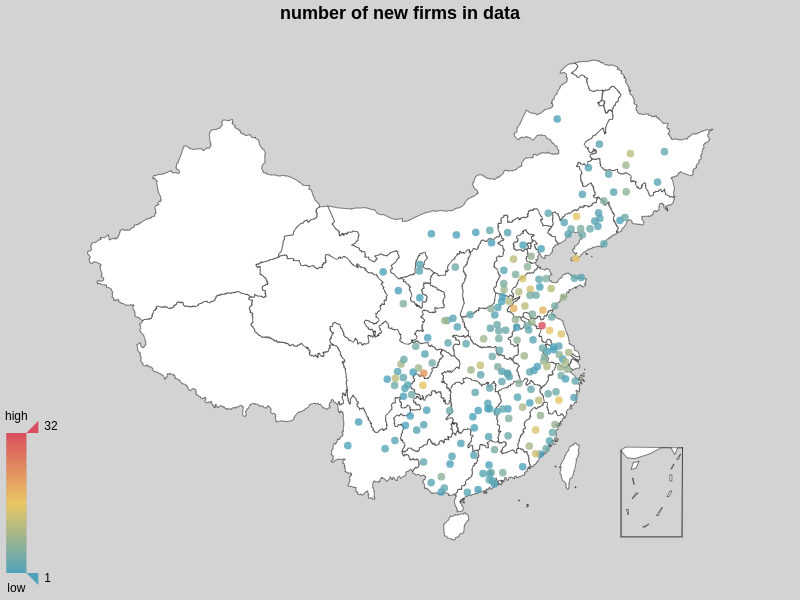
\includegraphics[scale=0.24]{\graphs/number of new firms in data.png}
        \label{firm_city_map}
    \end{figure}
\end{frame}

\begin{frame}{Data}
    \begin{itemize}
        \item More than 80\% of firms have output level have out put level between 5 million and 250 million
              yuan per year, and most of the firms buy land with price below 3 million yuan per hectare.
    \end{itemize}
    \begin{figure}[H]
        \centering
        \caption*{Sample distribution of output level and land price}
        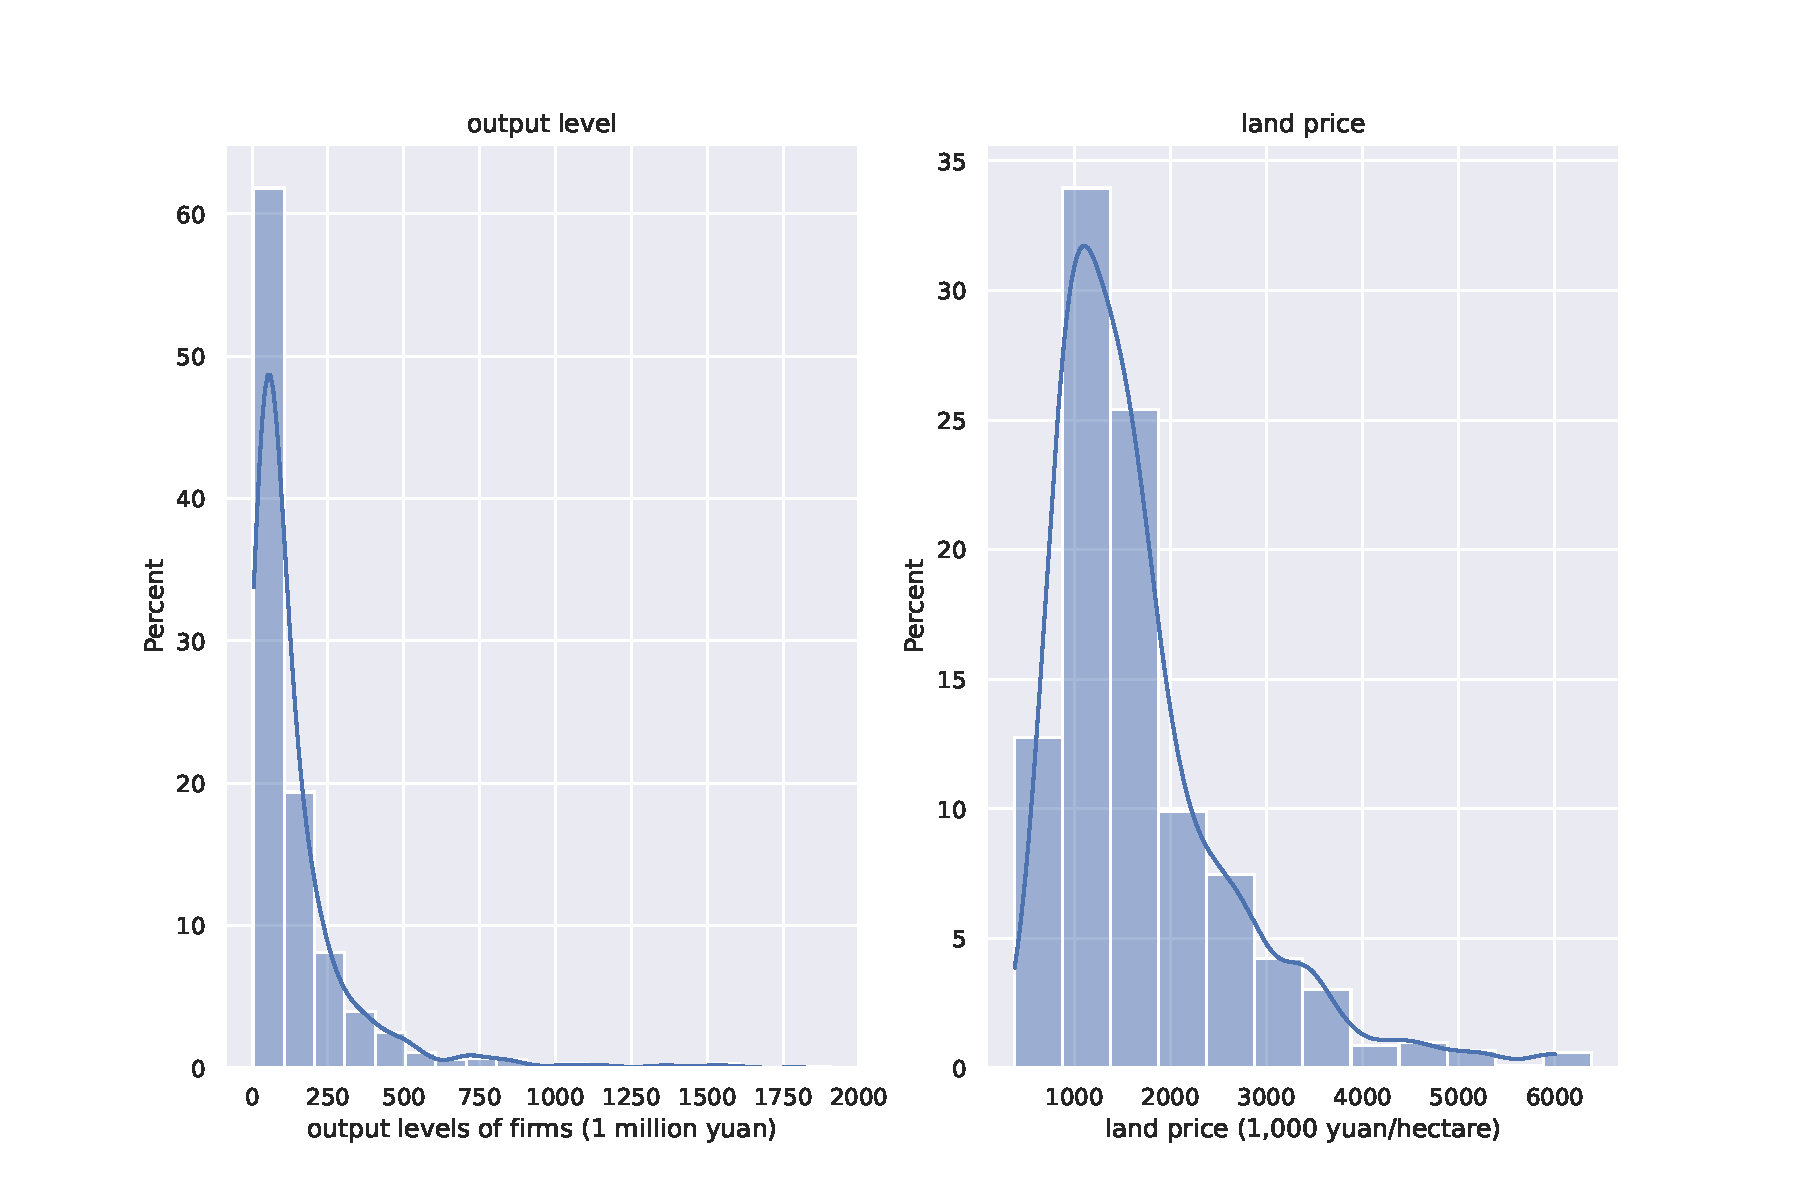
\includegraphics[scale=0.3]{\graphs/data_distribution.pdf}
        \label{distribution of output and price}
    \end{figure}
\end{frame}


\section{Estimation}
\subsection{Settings for Estimation}

\begin{frame}{Settings for Estimation}
    \begin{table}[H]
        \caption*{Inputs in the Bertrand Game model}
        \centering
        \resizebox{\textwidth}{!}{
            \begin{tabular}{ccccc}
                \toprule
                {\ul}      & {Name }        & {Interpretation}
                           & {Source}       & {Value/Range/Formula}
                \\ \midrule
                Parameters & $\beta$        & governments' revenue share
                           & estimation     & $[0, 2]$
                \\
                           & $\sigma$       & scale parameter in the distribution of
                $\varepsilon_{ik}$
                           & estimation     & $(0, 1000]$
                \\
                           & $\alpha$       & capital income share
                           & calibration    & $\{0.33, 0.5, 0.67\}$
                \\ \midrule
                Variables  & $Y_i$          & output level of firm
                           & data           &
                \\
                           & $L_i$          & number of workers in the firm
                           & data           &
                \\
                           & $T_i$          & area of land usage
                           & data           &
                \\         & $w_k$       & city average wage
                           & data           &
                \\
                           & $B_i$          & firm's characteristic
                           & data           & $L_i w_{k^*}^{\alpha}$
                \\
                           & $\mathbf{C}_i$ & firm's choice set
                           & random draws   & $|\mathbf{C}_i| = 3, 4, 5$
                \\
                           & $p^{i}_{obs}$  & observed land price for the firm
                           & data           &
                \\
                           & $p^{i}_{min}$  & the minimum of possible land price
                           & data           & $\max\{0, ~p^{i}_{obs} - 2000\}$
                \\
                           & $p^{i}_{max}$  & the maximum of possible land price
                           & data           & $p^{i}_{obs} + 2000$
                \\
                \bottomrule
            \end{tabular}}
    \end{table}

\end{frame}

\subsection{Moment Conditions}
\begin{frame}{Moment Conditions}
    \begin{itemize}
        \item I use the method of simulated moments (MSM) to estimate $\theta = (\beta, \sigma)$.
        \item The information of firm $i$ is $Q_i \equiv \{Y_i, T_i, B_i\}$, all the
              parameters is denoted by $\theta = (\alpha, \beta, \sigma)$. And $\theta_0$ are the true parameters.
        \item Define $x_i \equiv [p_i, p_i^2]^{'}$,
              and denote the conditional first and second-order moments of land price
              by $h(x_i; \theta_0) \equiv E(x_i|Q_i;\theta_0)$.
              By the definition of conditional land price:
              %\useshortskip
              \begin{equation*}
                  E[x_i - h(Q_i; \theta_0)|Q_i] = 0
              \end{equation*}
        \item I choose
              the instrument variables vector $Z_i = [1, Y_i, T_i, Y_i \times T_i]^{\prime}$
              for its simplicity.
              And the moment conditions are:
              %\useshortskip
              \begin{equation*}
                  E[Z_i \otimes \big(x_i - h(Q_i; \theta_0)\big)] = 0
              \end{equation*}
    \end{itemize}
\end{frame}

\subsection{Numerical Methods for Estimation}
\begin{frame}{Numerical Methods for Estimation}
    \begin{itemize}
        \item I use a two-step method (estimating the optimal weighting matrix)
              to get the estimates and standard errors.
        \item Grid search + Quasi-Newton method to find the minimizer of MSM objective.
    \end{itemize}
\end{frame}

\subsection{Estimation Results}
\begin{frame}{Estimation Results}
    \begin{itemize}
        \item The VAT rate is 17\%,
              the share of city government in VAT revenue is 25\%, and the back-of-envelop
              calculation shows that the city government's revenue share is at most
              $5 \times 80\% \times 17\% \times 25\% = 0.17$, which is 38\% of
              $\hat{\beta} \approx 0.45$ ($80\%$ is an overestimated added value-output ratio).
    \end{itemize}
    \begin{table}[H]
        \centering
        \caption*{Estimates of Parameters ($3 \leq |\mathbf{C}_i| \leq 5$)}
        \label{table: estimates (min_size=3 max_size=5 margin=2000)}
        \begin{tabular}{cccc}
            \toprule
            Calibrated $\alpha$ & Parameters & Estimates & Standard Error \\
            \midrule
            0.33                & $\beta$    & 0.512     & 0.043          \\
                                & $\sigma$   & 172.246   & 24.058         \\
            \midrule
            0.5                 & $\beta$    & 0.453     & 0.032          \\
                                & $\sigma$   & 178.301   & 25.102         \\
            \midrule
            0.67                & $\beta$    & 0.462     & 0.034          \\
                                & $\sigma$   & 182.761   & 24.920         \\
            \bottomrule
        \end{tabular}
    \end{table}


\end{frame}

\subsection{Fit of the Model}
\begin{frame}{Fit of the Model}
    \begin{figure}[H]
        \centering
        \caption*{Comparison of distribution of real land prices and simulated land prices}
        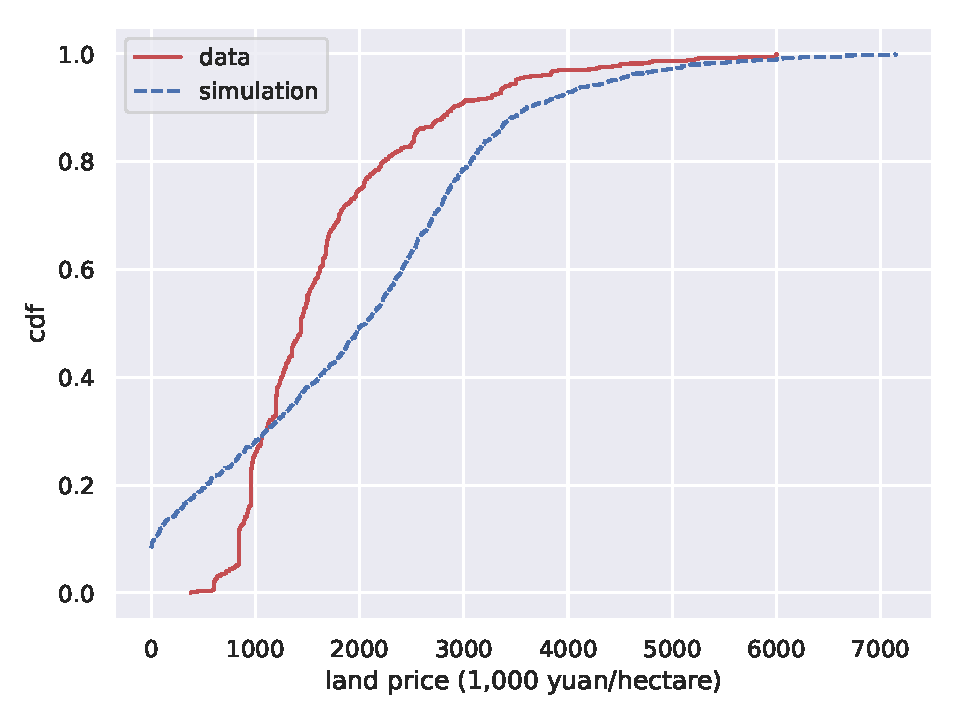
\includegraphics[scale=0.5]{\graphs/cdf_data_sim.pdf}
        \label{price distribution}
    \end{figure}
\end{frame}


\section{Counterfactual Analysis}
\subsection{Allocation Efficiency}
\begin{frame}{Allocation Efficiency}
    \begin{itemize}
        \item I fix land prices in the whole country,
              and calculate the probability of getting firms for advantaged cities in
              the Bertrand game.
        \item  The impact
              of fiscal competition on the locations of firms (allocation efficiency)
              is very small.
    \end{itemize}
    \begin{figure}[H]
        \centering
        \caption*{The empirical CDF of the probability of getting the firm for advantaged cities}
        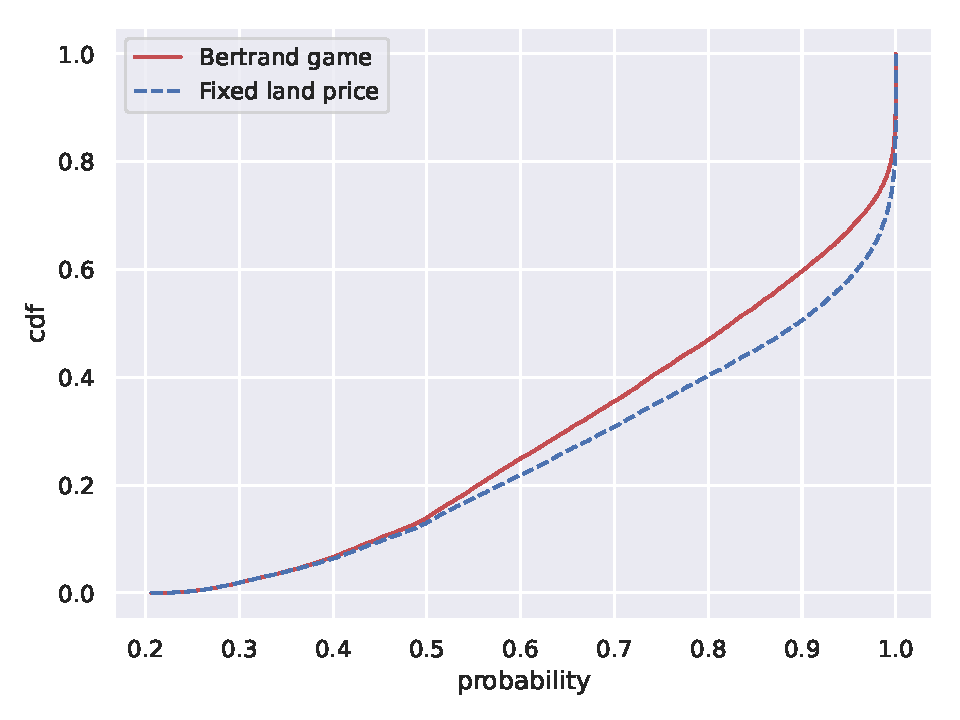
\includegraphics[scale=0.45]{\graphs/allocation_efficiency.pdf}
    \end{figure}
\end{frame}


\subsection{Impacts of fiscal centralization}
\begin{frame}{Impacts of fiscal centralization}
    \begin{itemize}
        \item I consider “fiscal centralization” after 2013 reflected by the decrease of $\beta$.
        \item If $\beta$ decreases by 25\%, the spillover effects of
              attracting firms are still sufficiently large, and the rise of land prices is limited.
    \end{itemize}
    \begin{figure}[H]
        \centering
        \caption*{Change of land price distribution due to decrease of $\beta$}
        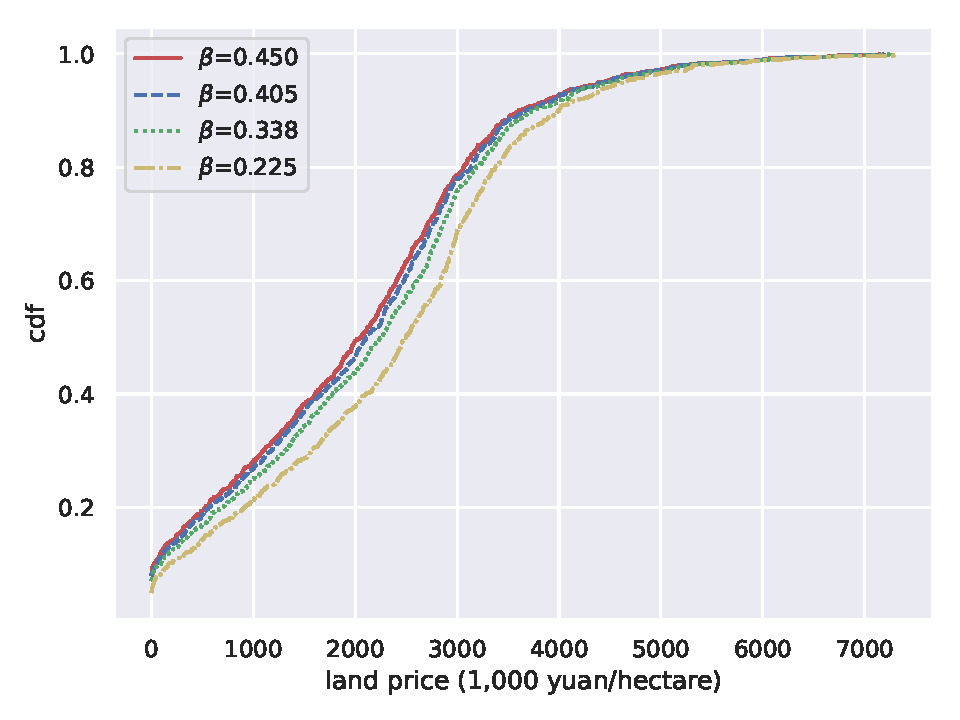
\includegraphics[scale=0.45]{\graphs/cdf_beta_decrease.pdf}
    \end{figure}
\end{frame}


\begin{frame}{Impacts of the Rising Wage Level}
    \begin{itemize}
        \item  I consider the impacts of rising urban wages in China after the late 2000s
              on the land price.
        \item The average land price
              increases as the wage level increases, but the increase is not sharp.
    \end{itemize}
    \begin{figure}[H]
        \centering
        \caption*{Change of land price distribution due to increase of wage}
        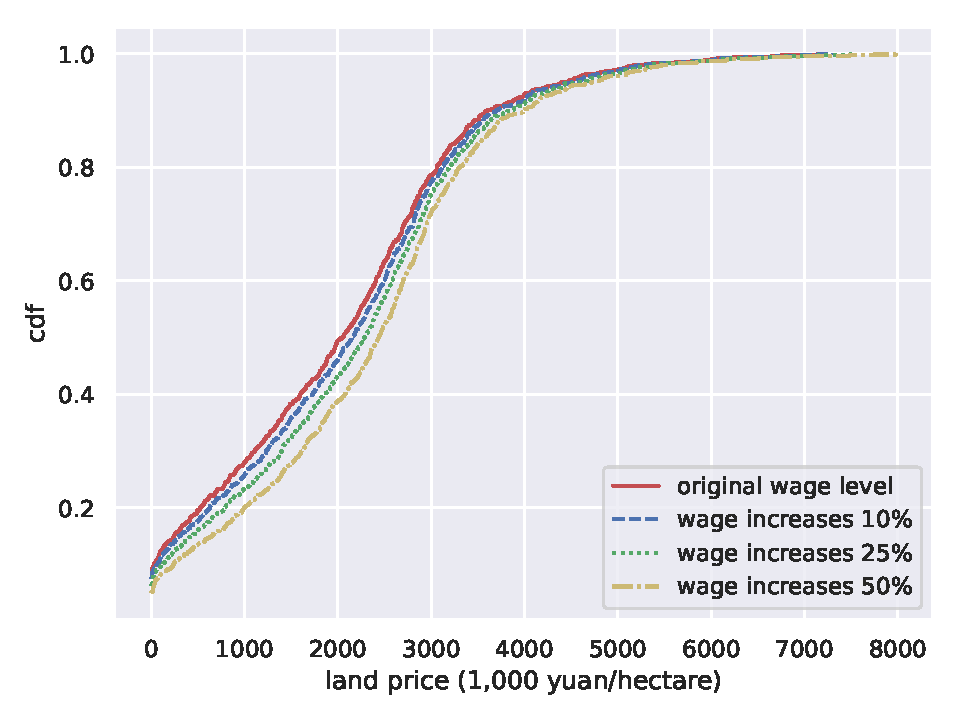
\includegraphics[scale=0.45]{\graphs/cdf_wage_increase.pdf}
    \end{figure}

\end{frame}

\section{Conclusion}
\begin{frame}{Conclusion}
    \normalsize
    \begin{itemize}
        \item Local governments can get huge benefits from attracting industrial firms.
              And the ratio of fiscal revenue to firms' output is much higher than the official tax rate.
        \item The major tool for the fiscal competition:
              selling industrial land at low prices cannot improve the allocation efficiency of output
              but waste a lot of potential land-selling revenue.
        \item The real potential benefits of fiscal competition can only be the case that more
              firms (or output level) are created due to the lower production cost
              induced by the efforts of local governments to attract firms. But this
              issue is beyond the scope of the model.
        \item Fiscal centralization poses potential challenges to the mode of fiscal competition.
    \end{itemize}
\end{frame}

% \section*{Reference} no need to start a new section
\begin{frame}[allowframebreaks]{References}
    \bibliography{reference}
\end{frame}

\end{document}